\documentclass{beamer}
%AMDG
\usepackage{amsmath, amsthm, amssymb}
\usepackage{hyperref}
\usepackage[slovene]{babel}
\usepackage[utf8]{inputenc}
\usepackage[T1]{fontenc}
\usepackage{epigraph}
\usepackage{pdftexcmds}
\usepackage{fancyref, nameref}
\usepackage{epigraph}
\usepackage{cleveref}
\usepackage{verbatim}
%\usepackage{enumitem}
\usepackage{multicol}
\usepackage[nomessages]{fp}
\usepackage{fancyhdr}
\usepackage{multirow}
\usepackage{mathtools}

\usepackage{tikz}

\usetheme{Warsaw}

\newenvironment{remark}
{\textbf{Opomba:}}
{}

\newcommand{\subscript}[2]{$#1 _ #2$}

\newcommand{\twopartdef}[4]
{
	\left\{
		\begin{array}{ll}
			#1 & \mbox{; } #2 \\
			#3 & \mbox{; } #4
		\end{array}
	\right.
}


%operatorji
\newcommand{\ord}{\ensuremath{\operatorname{red}}} % red grupe/elementa
\newcommand{\Mod}[1]{ \ (\text{mod}\ #1)}

\beamertemplatenavigationsymbolsempty

\setbeamerfont{page number in head/foot}{size=\large}
\setbeamertemplate{footline}[frame number]

\usetheme{Antibes}

\author{Kralj Samo, Koprivec Filip}

\title{Mreže}
\institute{FMF}
\date{\today}

\begin{document}
\begin{frame}
	\titlepage
\end{frame}

\begin{frame}
	\tableofcontents
\end{frame}

\begin{frame}
\section{Osnovne definicije}
\frametitle{Urejenost}

\begin{definition}
Naj bo $\mathcal{L}$ množica, relacija $\leq$ je \textbf{(šibka) delna urejenost}, če je
\begin{itemize}
\item refleksivna ($a \leq a$)
\item antisimetrična ($a \leq b \land b \leq a \implies a = b$)
\item tranzitivna ($a \leq b \land b \leq c \implies a \leq c$)
\end{itemize}
\end{definition}

\begin{remark}
Občasno smo nekoliko "šlampasti" in za lažjo predstavljivost uporabimo tudi relacijo $\geq$, ki jo definiramo kot $a \geq b \iff b \leq a$
\end{remark}

\begin{block}{Dogovor}
Naj bo $\mathcal{L}$ množica urejena z relacijo delne urejenosti $\leq$ in $x,y \in \mathcal{L}$
\end{block}

\end{frame}

\begin{frame}

\frametitle{Supremum in infimum}

\begin{definition}
$S$ je \textbf{supremum} $x$ in $y$, če velja: 
\begin{itemize}
\item $S \geq x \land S \geq y$ (Zgornja meja)
\item $\forall S' \in \mathcal{L} \implies (S' \geq x \land S' \geq y \implies S \leq S')$ (Je najmanjša zgornja meja)
\end{itemize}
označimo: $S = x \lor y$ 
\end{definition}

\begin{definition}
$s$ je \textbf{infimum} $x$ in $y$, če velja: 
\begin{itemize}
\item $s \leq x \land s \leq y$ (Spodnja meja)
\item $\forall s' \in \mathcal{L} \implies (s' \leq x \land s' \leq y \implies s' \leq s)$ (Je največja spodnja meja)
\end{itemize}
označimo: $s = x \land y$ 
\end{definition}

\end{frame}

\begin{frame}
\begin{definition}
Množica $\mathcal{L}$ je \textbf{linearno urejena}, če za poljubna $x,y$ velja $x \leq y$ ali  $y \leq x$ 
\end{definition}

\begin{definition}
Množica $\mathcal{L}$ je \textbf{mreža}, če ima poljuben par $x,y$ infimum in supremum.
\end{definition}

\end{frame}

\begin{frame}
\begin{columns}
\begin{column}{2cm}
  \begin{figure}
  \centering
  \begin{tikzpicture}[scale=1]
    \node (a) at (0,0) {$a$};
    \node (b) at (-1,-1) {$b$};
    \node (c) at (-1,-2) {$c$};
    \node (d) at (0,-3) {$d$};
    \node (e) at (1,-1.5) {$e$};
    \draw (a) -- (b) -- (c) -- (d) -- (e) -- (a);
  \end{tikzpicture}
  \end{figure}
\end{column}

\begin{column}{2cm}
  \begin{figure}
  \centering
  \begin{tikzpicture}[scale=1]
    \node (a) at (0,0) {$a$};
    \node (b) at (-1,-1) {$b$};
    \node (c) at (-1,-2) {$c$};
    \node (d) at (0,-3) {$d$};
    \node (e) at (1,-1.5) {$e$};
    \node (f) at (1.5,-2.5) {$f$};
    \draw (a) -- (b) -- (c) -- (d) -- (e) -- (a);
    \draw (e) -- (f);
  \end{tikzpicture}
  \end{figure}
\end{column}

\end{columns}
\end{frame}


\begin{frame}
\begin{center}
$\mathbb{N}, |$
\end{center}
\begin{figure}
\centering
\begin{tikzpicture} % should make python program :(
  \node (one) at (1,4) {$0$};
  \node (two) at (-3,0) {$2$};
  \node (three) at (-1,0) {$3$};
  \node (five) at (2,0) {$5$};
  \node (rest_primes) at (4,0) {$\dots$};
  \node (rest_primes_2) at (5,0) {$\dots$};
  \node (rest_second) at (4,2) {$\dots$};
  \node (rest_second_2) at (5,2) {$\dots$};
  
  \node (four) at (-3,2) {$4$};
  \node (six) at (-2,2) {$6$};
  \node (nine) at (-1,2) {$9$};
  \node (ten) at (0,2) {$10$};
  \node (fifteen) at (1, 2) {$15$};
  \node (twentyfive) at (2,2) {$25$};
  
  \node (zero) at (1,-2) {$1$};
  
  \draw (zero) -- (two) -- (six) -- (three) -- (fifteen) -- (five) -- (zero) -- (rest_primes);
  \draw (rest_primes_2) -- (zero) -- (three);


  \draw (two) -- (four);
  \draw (three) -- (nine);
  \draw (two) -- (ten) -- (five);
  \draw (five) -- (twentyfive);
  \draw[loosely dotted] (four) -- (one);  
  \draw[loosely dotted] (six) -- (one);  
  \draw[loosely dotted] (nine) -- (one);  
  \draw[loosely dotted] (ten) -- (one);
  \draw[loosely dotted] (fifteen) -- (one);  
  \draw[loosely dotted] (twentyfive) -- (one);  
  \draw[loosely dotted] (rest_primes) -- (rest_second) -- (one);
  \draw[loosely dotted] (rest_primes_2) -- (rest_second_2) -- (one);
  
\end{tikzpicture}
\end{figure}

primeri in neprimeri mrež, hassejev diagram

naravna števila, naraqvna za deljivost, potenčna za vsebovanost

\end{frame}

\begin{frame}
\begin{definition}
Mreža $\mathcal{L}$ je polna, če za poljubno $\mathcal{A} \subseteq \mathcal{L}$ obstajata infimum in supremum za $\mathcal{A}$.
\end{definition}
Primeri(omejena lienarna), potenčna..., protiprimeri(realna), podgrupe dane množice

\end{frame}

\begin{frame}
\begin{block}{Zakoni v mrežah}
\begin{itemize}
\item $x \lor x = x$, $x \land x = x$ (Idempotentnost)
\item $x \lor y = y \lor x$, $x \land y = y \land x$ (Komutativnost)
\item $(x \lor y) \lor z = x \lor (y \lor z)$\\ $(x \land y) \land z = x \land (y \land z)$ (Asociativnost)
\item $ x \lor (x \land y) = x$\\ $x \land (x \lor y) = x$ (Absorbcija)
\end{itemize}
\end{block}
\end{frame}


\begin{frame}
\begin{proof}
Naj bo $a = (x \lor y) \lor z$ in $b = x \lor (y \lor z)$ \\ \pause
Iz definicje ali sledi $a \geq z$ in $a \geq (x \lor y)$ in torej $a \geq x, a \geq y$ \\ \pause
Potem velja tudi $a \geq (y \lor z)$ in $a \geq x \lor (y \lor z)$ torej $a \geq b$\\ \pause
Na skoraj enak naredimo iz druge strani in dobimo $b \geq a$, ker pa je zaradi antisimetričnosti relacije mogoče zgolj, kadar velja $a=b$
\end{proof}
\end{frame}

\begin{frame}
\begin{proof}
Iz definicije ali vemo $x \leq (x \lor y)$ in $x \leq x$ torej $x \leq x \land (x \lor y)$\\ \pause
Iz definicije in pa sledi $x \geq x \land (x \lor y)$\\ \pause
Torej $x \leq x \land (x \lor y)$ in $x \geq x \land (x \lor y)$, dobimo $x = x \land (x \lor y)$

\end{proof}
\end{frame}


\begin{frame}
\begin{theorem}
Če imamo množico $\mathcal{L}$, za katero sta definirani operaciji $\lor, \land$ in če za te dve operacji veljajo zgornji zakoni, potem je ta množica mreža.
\end{theorem}
\end{frame}

\begin{frame}

\begin{block}{Dokaz}
Najprej definiramo relacijo, naj za $x,y \in \mathcal{L}$ velja $x \leq y \iff x \land y = x$\\ in preverimo, da je to delna urejenost \\ \pause
Refleksivnost: \pause$x \land x = x$ torej $x \leq x$\\ \pause
Antisimetričnost: \pause $x \leq y$ in $y \leq x$, torej $x \land y = x$ in $y \land x = y$, uporabimo komutativnost in dobimo $x = y$\\ \pause
Tranzitivnost: \pause $x \leq y$ in $y \leq z$ torej velja $x = x \land y$ in $y = y \land z$ \\ \pause
Namesto $y$ uporabimo $y \land z$ in dobimo $x = x \land (y \land z) = (x \land y) \land z = x \land z$ torej \pause $x \leq z$ \\ \pause
Preverimo še, da velja $x \land y = x \iff x \lor y = y$\\ \pause
Uporabimo zadnji zakon in $x \lor b = (x \lor y) \land y = b$ in identično v drugo smer.

\end{block}

\end{frame}


\begin{frame}
\begin{proof}
Preveriti moramo še infimume in supremume\pause, poglejmo si samo supremum\\ \pause
Sama od sebe se nam kot zgornja meja $x$ in $y$ ponuja $x \lor y$, ki je očitno zgornja meja \\ \pause%ker smo obstoj relacije že dokazali, lahko sedaj uporabljamo vse kar nam de
Naj bo $z$ neka zgornja meja $x,y$, $x \lor z = y \lor z = z$\\ \pause
Dobimo $(x \lor y) \lor z = x \lor (y \lor z) = x \lor z = z$, kar pomeni, da $x \lor y \leq z$, torej je $x \lor y$ natančna zgornja meja. 
\end{proof}
\end{frame}

\begin{frame}

\begin{block}{}
Naravno se pojavi vprašanje, ali za operaciji v mrežah obstaja kakšne vrste enota ali celo inverz.
\end{block}

\begin{definition}
Če v mreži obstaja največji element, potem ta element označimo z $1$ ($\forall x \in \mathcal{L}. \ x \leq 1$)
\end{definition}

\begin{definition}
Če v mreži obstaja najmanjši element, potem ta element označimo z $0$ ($\forall x \in \mathcal{L}. \ x \geq 0$)
\end{definition}

\end{frame}

\begin{frame}
\begin{block}{}
Če v mreži obstajata $0$ in $1$ potem velja:
\begin{itemize}
\item $x \lor 1 = 1$
\item $x \lor 0 = x$
\item $x \land 0 = 0$
\item $x \land 1 = x$
\end{itemize}
\end{block}

Primeri
\end{frame}

\begin{frame}
\begin{definition}
V mreži z elementoma $0$ in $1$ elementa $x$ in $x'$ imenujemo \textbf{komplementarna}, če velja:
\begin{itemize}
\item $x \lor x' = 1$
\item $x \land x' = 0$
\end{itemize}
\end{definition}

\begin{definition}
Mrežo, v katri poljubnemu $x$ pripada \textbf{vsaj} en komplement imenujemo \textbf{komplementarna mreža}.
\end{definition}

\end{frame}

\begin{frame}
Primeri(vektorski prostor na vsebovanost), komplementi
\end{frame}

\begin{frame}
\begin{definition}
Neprazna množica $\mathcal{M} \subseteq \mathcal{L}$ je \textbf{podmreža}, če je tudi sama mreža za isti operaciji in se na njih ujema. Povedano drugače $x \lor y \in \mathcal{M}$ in $x \land y \in \mathcal{M}$
\end{definition}
\end{frame}

\begin{frame}
Med dvema je spet podmreža
\end{frame}


\begin{frame}
\begin{columns}
\begin{column}{5cm}
\begin{center}
$\{0,1\}, \subseteq$
\end{center}
\begin{figure}
\centering
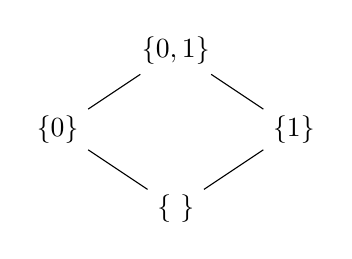
\begin{tikzpicture}[scale=0.5]
  \node (one) at (0,2) {$\{0,1\}$};
  \node (a) at (-3,0) {$\{0\}$};
  \node (d) at (3,0) {$\{1\}$};
  \node (zero) at (0,-2) {$\{ \ \}$};
  \draw (zero) -- (a) -- (one)  -- (d) -- (zero);
\end{tikzpicture}
\end{figure}
\end{column}

\begin{column}{5cm}
\begin{center}
$\{1,2,3,6\}, |$
\end{center}
\begin{figure}
\centering
\begin{tikzpicture}[scale=0.5]
  \node (one) at (0,2) {$6$};
  \node (a) at (-3,0) {$3$};
  \node (d) at (3,0) {$2$};
  \node (zero) at (0,-2) {$1$};
  \draw (zero) -- (a) -- (one)  -- (d) -- (zero);
\end{tikzpicture}
\end{figure}
\end{column}
\end{columns}

\begin{block}{}
Mreži se zdita sumljivo podobni, ali lahko to kako posplošimo?
\end{block}

\end{frame}

\begin{frame}
\begin{definition}
Preslikava $f :\mathcal{L} \to \mathcal{L}'$ je \textbf{homomorfizem}, ča za poljubna $x,y \in \mathcal{L}$ velja:
\begin{itemize}
\item $f(x \lor y) = f(x) \lor f(y)$
\item $f(x \land y) = f(x) \land f(y)$
\end{itemize}
\end{definition}

%% Tukej je treba povedati zakaj


\begin{block}{funkcija za prej}
Funkcija za prej
\end{block}

\end{frame}

\begin{frame}
\begin{theorem}
Za nek homomorfizem $f$ velja $f(\mathcal{L})$ je podmreža $\mathcal{L}$.
\end{theorem}

\begin{remark}
Homomorfizem ohranja urejenost
\end{remark}
\end{frame}


\begin{frame}

\begin{theorem}
Bijektivni homomorfizem $f$, $f \mathcal{L} \to \mathcal{L}'$ je izomorfizem, če ohranja red v obeh smereh
\end{theorem}

\begin{proof}

\end{proof}

\end{frame}

\begin{frame}
\begin{block}{Red se mora ohranjati v obeh smereh}
Protiprimer
\end{block}
\end{frame}


\begin{frame}
\begin{definition}
Mreža je \textbf{distributivna}, če za $\lor$ in $\land$ veljata zakona:
\begin{itemize}
\item $(x \lor y) \land z = (x \land z) \lor (y \land z)$
\item $(x \land y) \lor z = (x \lor z) \land (y \lor z)$
\end{itemize}
\end{definition}


\begin{example}
linarana je distributivna
\end{example}

\end{frame}

\begin{frame}
\begin{theorem}
Če ima distributivna mreža $\mathcal{L}$ elementa $0,1$, potem ima vsak elementa največ en komplment (ni pa še zagotovljen obstoj komplementa)
\end{theorem}

\begin{proof}
Dokaz
\end{proof}

\end{frame}

\begin{frame}
Primerji (če ima vsak element komplement, potem samo slikaš samo obrnjeno)
\end{frame}

\begin{frame}% pa pridimo do mreže brez urejenosti
\begin{definition}
Kolobar, v katerem je vsak element idempotenten imenujemo \textbf{Boolov kolobar}.
\end{definition}
\end{frame}


\begin{frame}
\begin{theorem}
Boolov klobar je komutativen s karakteristiko $2$
\end{theorem}

\begin{proof}
Dokaza
\end{proof}
\end{frame}

\begin{frame}
\begin{block}{}
Definiramo operaciji $\lor, \land$ in pokažimo, da je to mreža
\end{block}
\end{frame}


\begin{frame}
\begin{definition}
Komplementarno in distributivno mrežo imenujemo \textbf{Boolova algebra}.
\end{definition}

\begin{block}{}
To ni algebra?????
\end{block}
\end{frame}

\begin{frame}
\section{Modulske mreže}
\begin{definition}
Mreža $\mathcal{L}$ je \textbf{modulska} mreža, če za $a \leq c$ velja:
$$(a \lor b) \land c = a \lor (b \land c)$$
\end{definition}
\end{frame}


\begin{frame}
test
\end{frame}


\end{document}
